% add ref biblio passive radar IEEE
\documentclass[compress,10pt]{beamer}
\usepackage{url,verbatim,amsmath}

\setbeamertemplate{background canvas}[vertical shading][bottom=white,top=structure.fg!25]
\usetheme{Hannover}
\setbeamertemplate{headline}{}
\setbeamersize{text margin left=0cm}
\graphicspath{{../../tutorials/plutosdr/2-PRN_on_PL/images/}{../gnuradioDays2019/}}

\beamertemplatefootpagenumber
\beamertemplatenavigationsymbolsempty
\definecolor{mygreen}{rgb}{0,0.6,0}

\usepackage{color}
\definecolor{grey}{rgb}{0.95,0.95,0.95}
\definecolor{keyword}{rgb}{0,0,0.95}
\definecolor{comment}{rgb}{0.95,0,0}
%\definecolor{include}{rgb}{0.55,0,0}
\definecolor{string}{rgb}{0,0.55,00.95}

\usepackage{listings}
\lstset{%backgroundcolor=\color{grey},
        language=C,
        numbers=left,
        numbersep=6pt,
        basicstyle=\tiny\ttfamily,
        extendedchars=true,
        tabsize=3,
        keywordstyle=\color{keyword}\bfseries,
        commentstyle=\color{comment},
%       includestyle=\color{include},
        stringstyle=\color{string}\itshape,
        columns=fullflexible,
        keepspaces=true
}

\setbeamertemplate{footline}{28 Nov 2019, Swiss Aeropole, Payerne (CH)}

\begin{document}
\date{November 28, 2019}
\author[G. Goavec- Merou \& al.]{Goavec-Merou, Jean-Michel Friedt\\
{\footnotesize
FEMTO-ST Time \& Frequency department, Besan\c con, France \\ 
}
Contact: {\tt \{gwenhael.goavec,jmfriedt\}@femto-st.fr} \\ \vspace{0.6cm}
\begin{center}
Slides at \\
\url{https://github.com/oscimp/oscimpDigital/tree/master/doc/tutorials/plutosdr/2-PRN_on_PL}\\\ \\ \ \\

\includegraphics[height=1cm]{logo_femto.pdf}\vspace{-1cm}
\end{center}
}
\title[]{OscImpDigital CPU-FPGA co-design framework in the context of satellite communication}

\begin{frame}
\titlepage
\end{frame}

%Software Defined Radio (SDR) provides a flexible framework for addressing multiple communication modes and reconfiguring a single hardware platform to match the requirements of several communication systems. Since the datarate is defined by communication bandwidth, maximizing sampling rate is often desirable if only to compensate for Doppler shift of the moving source, requiring a Field Programmable Gate Array (FPGA) as processing frontend between the Analog to Digital Converter (ADC) and general purpose Central Processing Unit (CPU). However, the hassle of developing on the FPGA compared to the flexible frameworks running on general purpose CPU, most significantly GNU Radio [0], drives the need to find the optimum boundary between FPGA and CPU processing defined by bandwidth and processing complexity. Addressing such challenges is met by the OscImpDigital [1] CPU-FPGA co-design framework in which a consistent set of signal processing blocks are provided to run on the FPGA, with the associated Linux module driver for configuring the selected blocks and libraries for accessing these drivers from userspace.

%We demonstrate the use of the OscImpDigital framework on the PlutoSDR SDR platform for receiving GPS signals. Since GPS signal is below thermal noise, pulse compression (correlating with each satellite Gold code) is mandatory to acquire the constellation, i.e. identifying the visible satellites and their Doppler shift. Rather than using the PlutoSDR as a basic SDR source with a communication bandwidth limited by the USB connection to the personal computer, all processing is run on the embedded Zynq System on Chip, making the most of the embedded FPGA and dual CPU for a fully autonomous processing system.

%[0] https://www.gnuradio.org/ and https://github.com/buildroot/buildroot/tree/master/package/gnuradio
%[1] https://github.com/oscimp/oscimpDigital/
%[2] https://github.com/oscimp/oscimpDigital/tree/master/doc/tutorials/plutosdr/2-PRN_on_PL

\section{GPS}
\begin{frame}\frametitle{Why SDR-based GNSS decoding~?}

\begin{enumerate}
\item Flexibility of adding new features without updating hardware
\item Beyond timing \& positioning: access to the raw I/Q stream
\begin{itemize}
\item basic physics (reflectometry)
\item security (phased array for spoofing detection)
\item 1575.42~MHz within range of the PlutoSDR (AD9363 + Zynq SoC)
\end{itemize}
\end{enumerate}

\vfill
\begin{center}
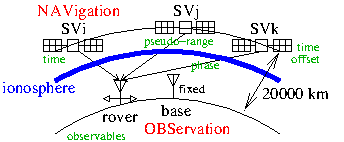
\includegraphics[width=.7\linewidth]{fig2}\\
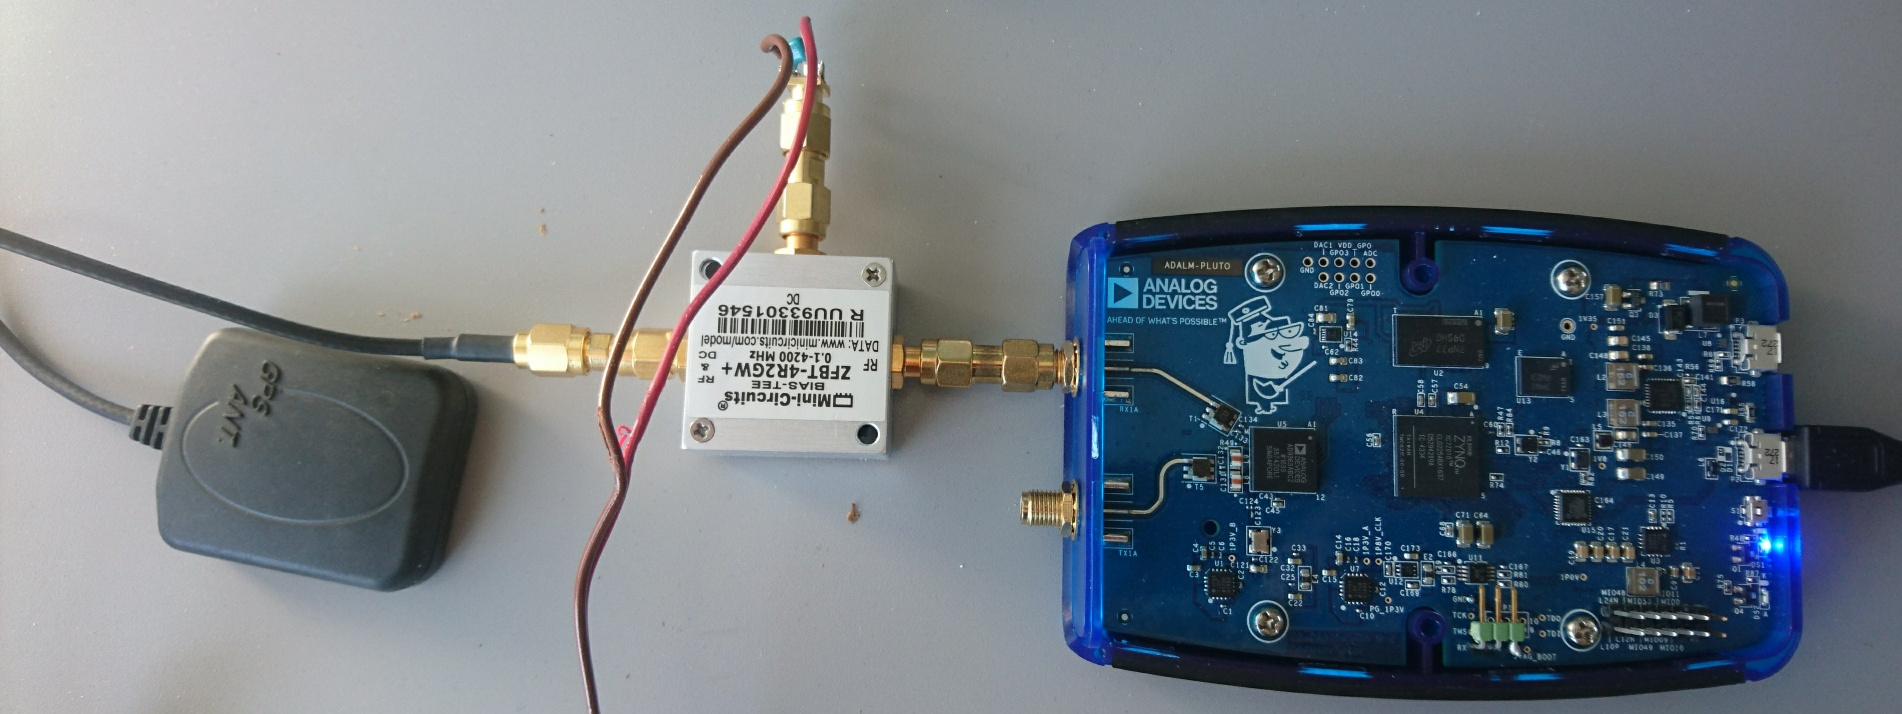
\includegraphics[width=.7\linewidth]{DSC_0279.JPG}
\end{center}

\end{frame}

\begin{frame}\frametitle{Basics on GPS encoding}

\begin{enumerate}
\item CDMA (Code Division Multiple Access): all satellites transmit on the same frequency
and their messages are encoded with individual orthogonal codes (Gold Codes)
\item Satellite identification: $xcorr(signal,code)$
\item Code orthogonality: $xcorr(code_i,code_j)=\delta_{i,j}$
\item Doppler shift: need to compensate for remote clock frequency wrt ground clock \& local clock
offset wrt remote atomic clocks
\end{enumerate}

\begin{center}
\only<1>{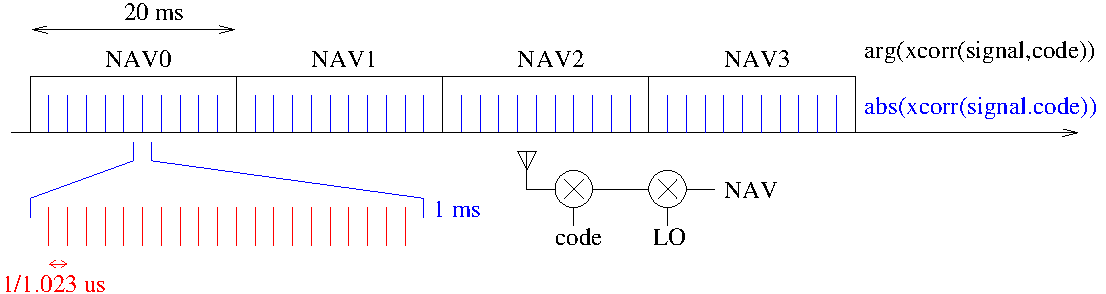
\includegraphics[width=\linewidth]{cdma}}
\only<2>{
\fbox{\parbox{0.8\linewidth}{
\begin{center}
Intensive use of correlations
\footnote{
Time-domain implementation on FPGA allows for pipelined computation as samples are collected
}
 \\$xcorr(x,y)(\tau)=\int x(t)y(t+\tau)dt$ \\or through the
convolution theorem: $FFT(xcorr(x,y)(\tau))=FFT(x)\cdot FFT(y^*)$ 
\end{center}
}}}
\end{center}

\end{frame}

\begin{frame}[fragile]\frametitle{Basics on GPS encoding}

GPS acquisition in 10~lines of Matlab program
\footnote{\tiny using the C/A code generator
\url{https://www.mathworks.com/matlabcentral/fileexchange/14670-gps-c-a-code-generator}} (two nested loops -- satellite number and frequency)

\begin{lstlisting}[language=Matlab]
pkg load signal
x=read_complex_binary(filename,1024*128); fs=1.023; % sampling rate in MHz
x=x-mean(x);
freq0=[-10.5e3:500:10.5e3];                         % Doppler range
time=[0:1/fs/1e6:length(x)/fs/1e6]';time=time(1:end-1);
for m=[1:31]                                        % loop on all satellites
   a=cacode(m,fs/1.023); a=a-mean(a);
   l=1;
   for freq=freq0                                   % loop on all frequency offsets
     mysine=exp(j*2*pi*(-freq)*time); 
     xx=x.*mysine;                                  % frequency shift the signal
     [u(l,m),v(l,m)]=max(abs(xcorr(a,xx,'none')));  % check for cross correlation max.
     l=l+1;
   end
end
\end{lstlisting}

\vspace{-0.70cm}
\begin{minipage}[t]{\linewidth}
\begin{minipage}{.49\linewidth}
{\footnotesize 
\begin{itemize}
\item Orbital mechanics: $Doppler\in [-5000 , 5000]$~Hz
\item Map xcorr max as a function of space vehicle number and frequency shift
\item When a satellite is visible, sharp xcorr peak when frequency offset is compensated for
\end{itemize}
}
\end{minipage}
\begin{minipage}{.49\linewidth}
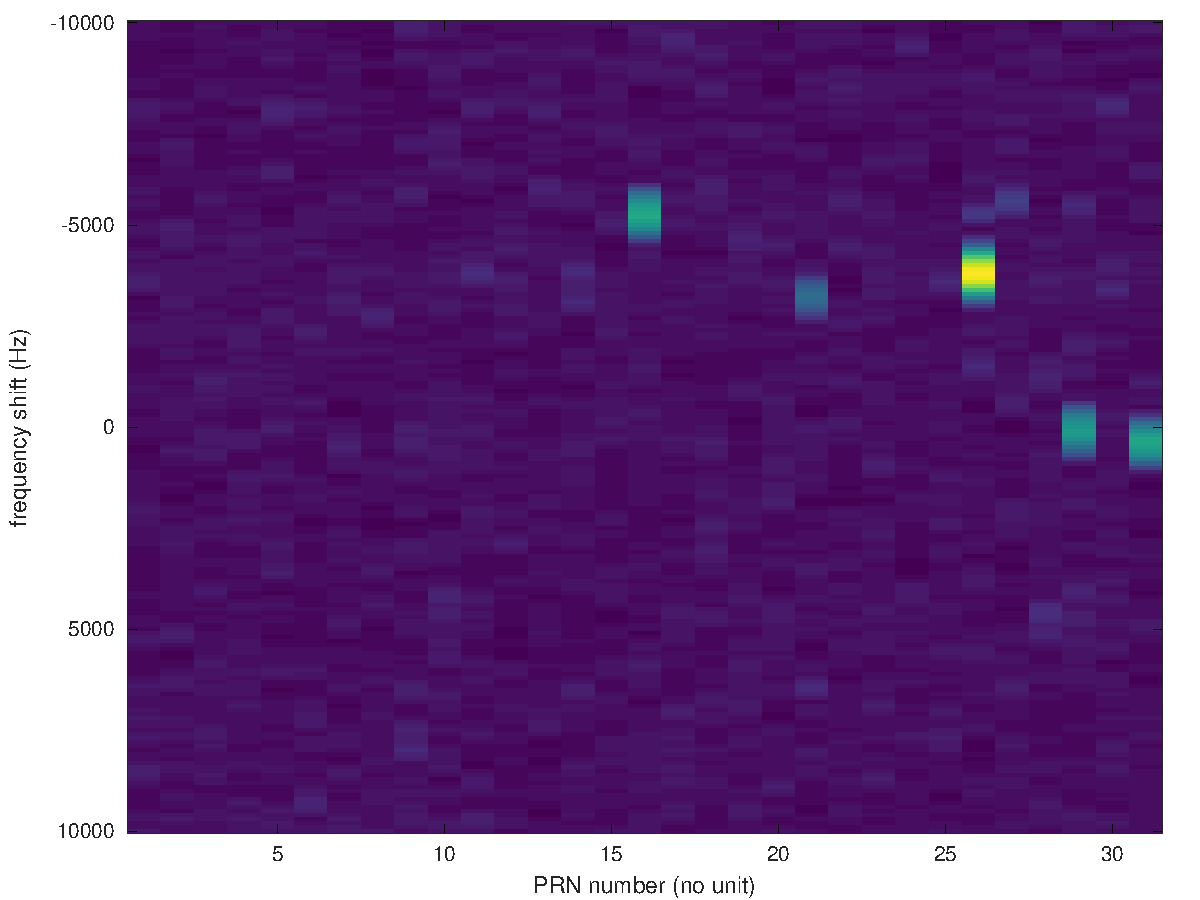
\includegraphics[width=\linewidth]{../190524gps_xcorr/gps_bin100Hz}
\end{minipage}
\end{minipage}
\end{frame}

\begin{frame}[fragile]\frametitle{Basics on GPS encoding}

GPS acquisition in 10~lines of Matlab program (single loop on space vehicle number)

\begin{lstlisting}[language=Matlab]
pkg load signal
x=read_complex_binary(filename,1024*128); fs=1.023; % sampling rate in MHz
x=x-mean(x);
freq0=[-10.5e3:500:10.5e3];                         % Doppler range
time=[0:1/fs/1e6:length(x)/fs/1e6]';time=time(1:end-1);
% doppler frequency shift matrix whose FFT is computed
doppler=exp(j*2*pi*freq0'*time');                   % 43x131072 matrix
data=ones(43,1)*x';
all=doppler.*data;                                  % Doppler-shifted data
allf=fft(all');
for m=[1:31]                                        % loop on all satellites
  a=cacode(m,fs/1.023);                             % CA code of satellite m
  a=[a zeros(1,length(all)-length(a))];             % zero padding
  a=a-mean(a);
  pattern=ones(43,1)*a;                             % 43x131072 matrix
  af=fft(pattern');
  correlation=ifft(af.*conj(allf))';
end
\end{lstlisting}

\vspace{-0.71cm}
\begin{minipage}[t]{\linewidth}
\begin{minipage}{.49\linewidth}
{\footnotesize 
\begin{itemize}
\item Replace loops (inefficient) with matrix multiplication
\item Parallelizing the frequency operations halves the computation time
\end{itemize}
}
\end{minipage}
\begin{minipage}{.49\linewidth}
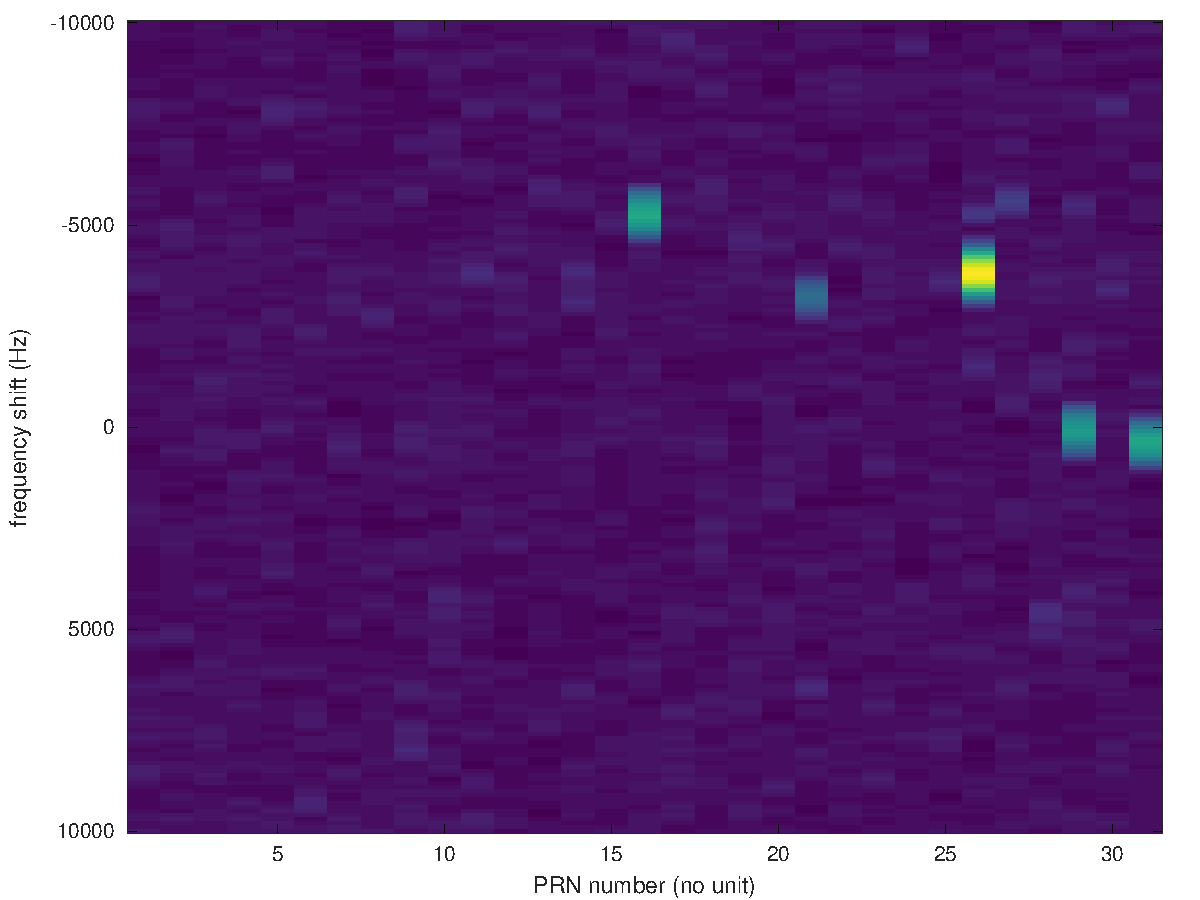
\includegraphics[width=\linewidth]{../190524gps_xcorr/gps_bin100Hz}
\end{minipage}
\end{minipage}
\end{frame}

\section{Embedded computation}
\begin{frame}[fragile]\frametitle{Using the embedded FGPA}

\begin{itemize}
\item
GNU/Octave implementation: 1 to 2 second/satellite \\
$\Rightarrow$ $\simeq$1~min for acquisition depending on frequency steps
\item The PlutoSDR Zynq is only used for data collection and transfer to the PC (bandwidth
limited by USB)
\item Preprocessing on the Zynq FPGA removes the communication bandwidth bottleneck
\item Making best use of the available resources on the embedded FPGA (PL)
\item Possible additional pre-processing on the embedded CPU (PS) running GNU Radio before sending
over USB
\end{itemize}

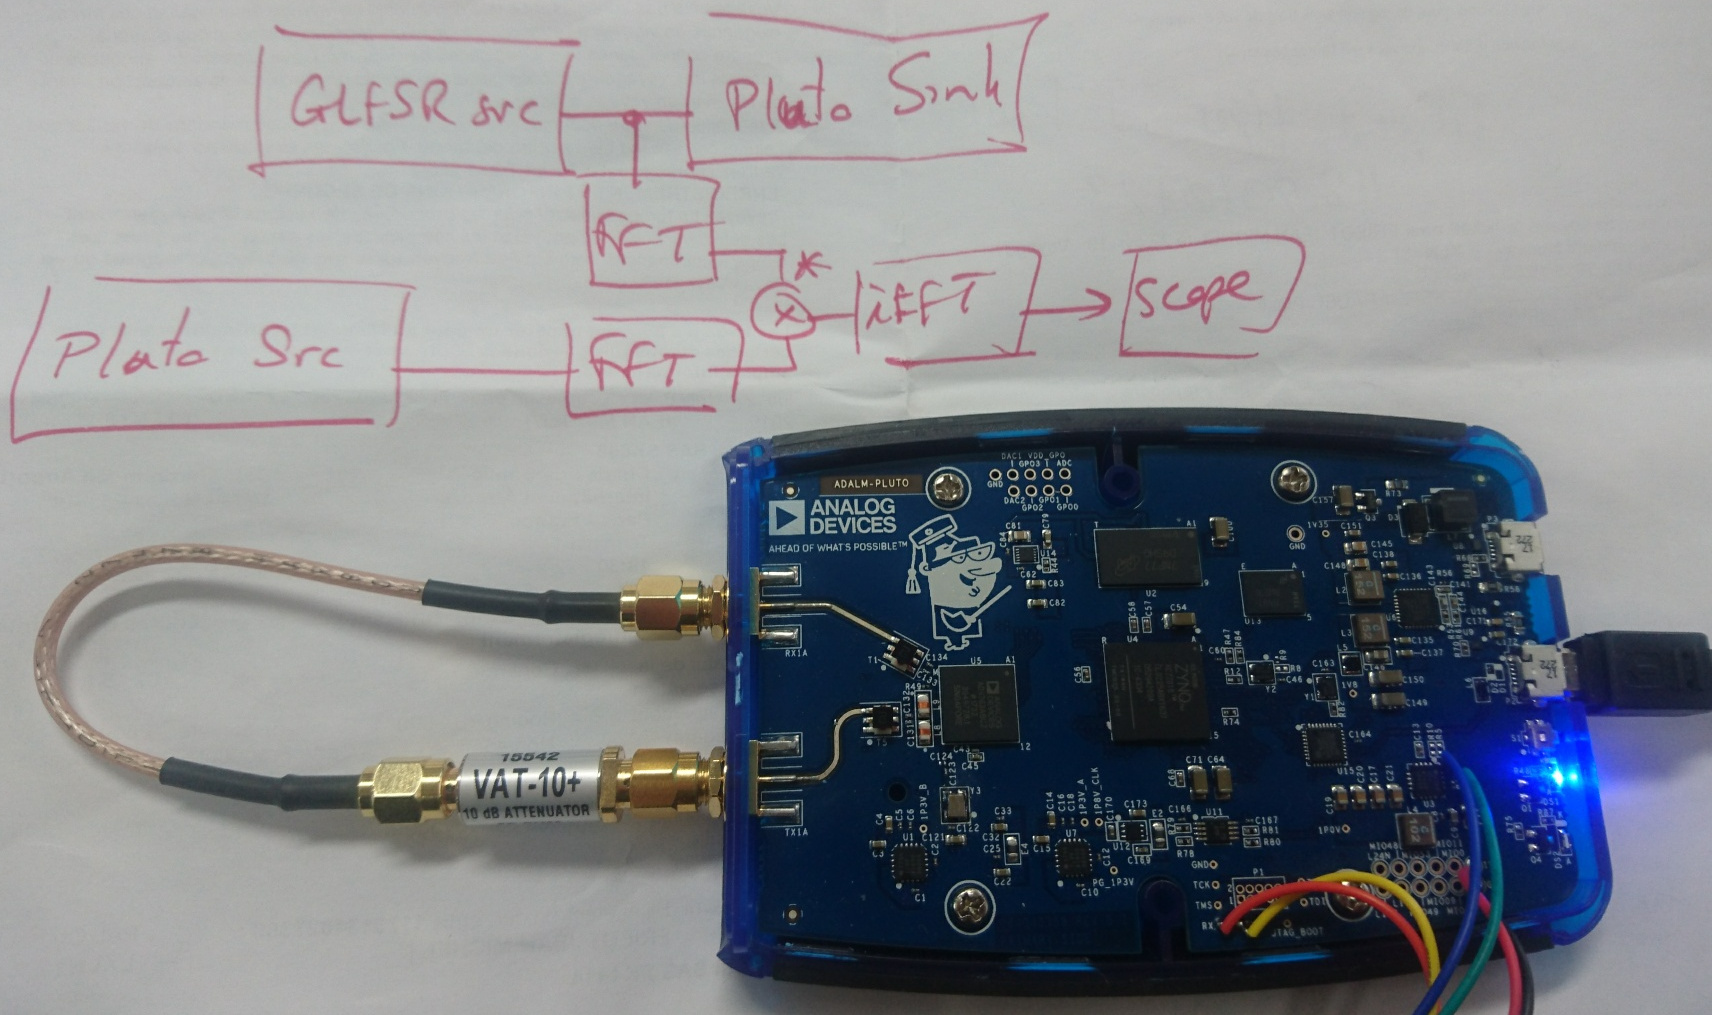
\includegraphics[width=.31\linewidth]{DSC_0275.JPG}
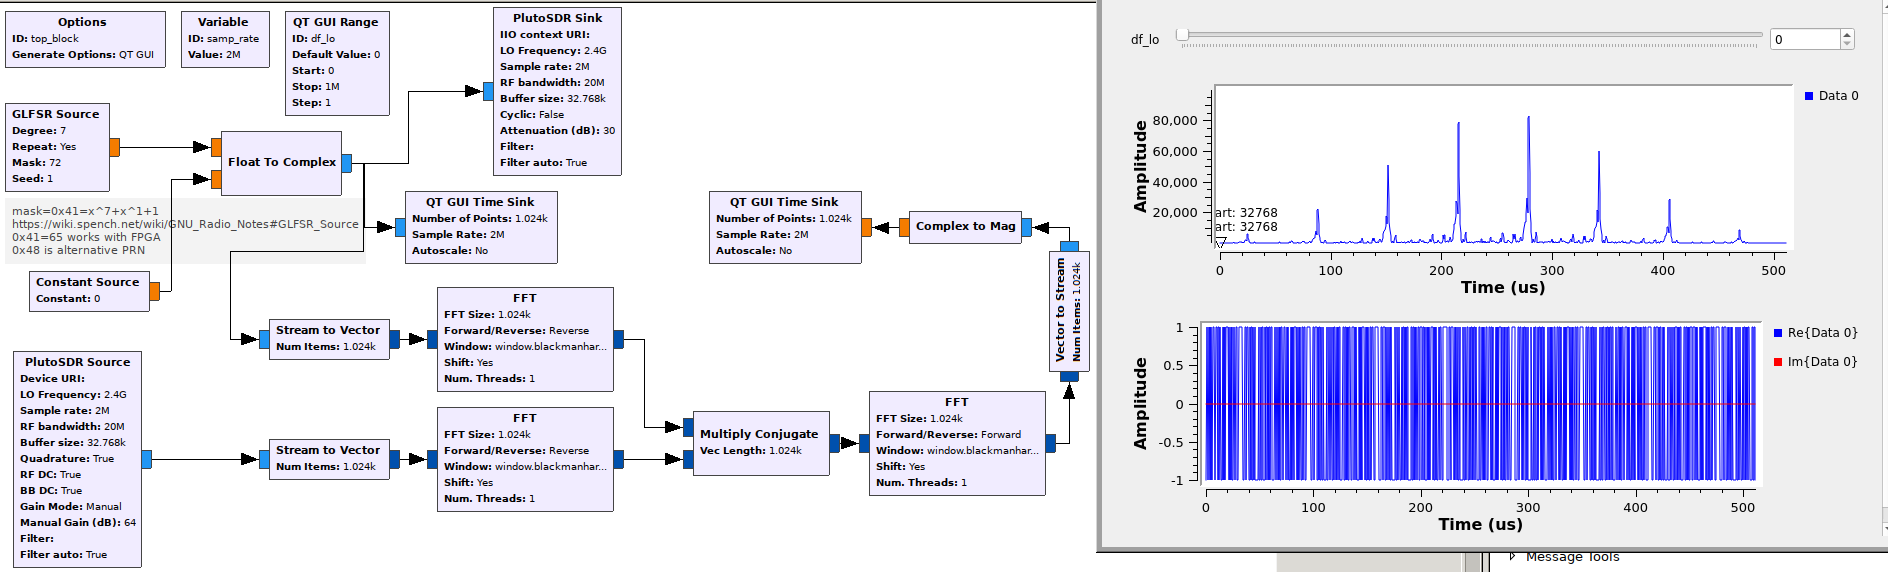
\includegraphics[width=.68\linewidth]{xcorr_pluto2}
\end{frame}

\begin{frame}[fragile]\frametitle{Principle}

\begin{center}
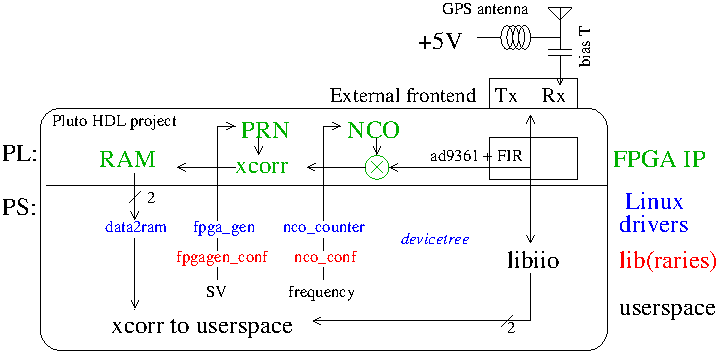
\includegraphics[width=\linewidth]{plutopluto-oscimpDigital-makerspace}
\end{center}

\begin{itemize}
\item PL: collect data from AD9363, frequency transposition (NCO), Gold Code generation \& correlation
\item PS: loop frequency, loop space vehicle number, fetch correlation, control AD9363 (libiio)
\end{itemize}

Complex interaction between FPGA processing blocks and processor userspace through
Linux drivers (modules)
\end{frame}

\section{OscimpDigital}

%\begin{frame}[fragile]\frametitle{The OscimpDigital framework}
%
%\vspace{-0.2cm}
%\hspace{-0.5cm}
%\begin{minipage}[t]{\linewidth}
%\begin{minipage}{0.8\linewidth}
%\hspace{-0.6cm}
%\begin{itemize}
%\item one algorithm $\Rightarrow$ one or more flavor (data type, performance vs.
%resources, ...): {\tt fpga\_ip} directory
%\item need to communicate between FPGA and CPU: {\tt linux\_driver} directory
%\item some IPs are widely used or complex to configure \\$\Rightarrow$ need
%to provide library with CPU code (reduce redundance, simplify application): {\tt
%liboscimp} in {\tt lib} directory.
%\end{itemize}
%\end{minipage}
%\begin{minipage}{0.1\linewidth}
%\center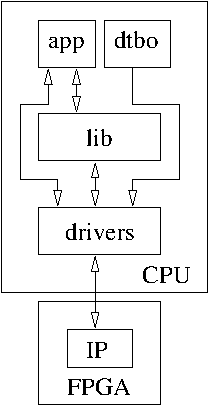
\includegraphics[width=2.6\textwidth]{./img/structureEco}
%\end{minipage}
%\end{minipage}
%\end{frame}


\frame{\frametitle{Oscimp EcoSystem}
Purpose: provide a coherent environment to create design (FPGA), and
application:

\vspace{-0.3cm}
\begin{minipage}[t]{\linewidth}
\begin{minipage}{0.6\linewidth}
\hspace{-0.2cm}
\begin{itemize}
\item blocks (IP) with algorithm level of implementation (FPGA);
\item GNU/Linux hierarchy compliance (driver/library/application);
\item tools to generate some files and scripts/Makefile to factorize most common
part.
\end{itemize}
\end{minipage}
\begin{minipage}{0.3\linewidth}
\center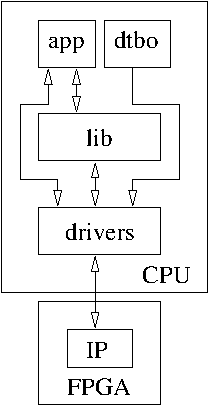
\includegraphics[width=0.7\textwidth]{./img/structureEco}
\end{minipage}
\end{minipage}
\vspace{-0.5cm}
\center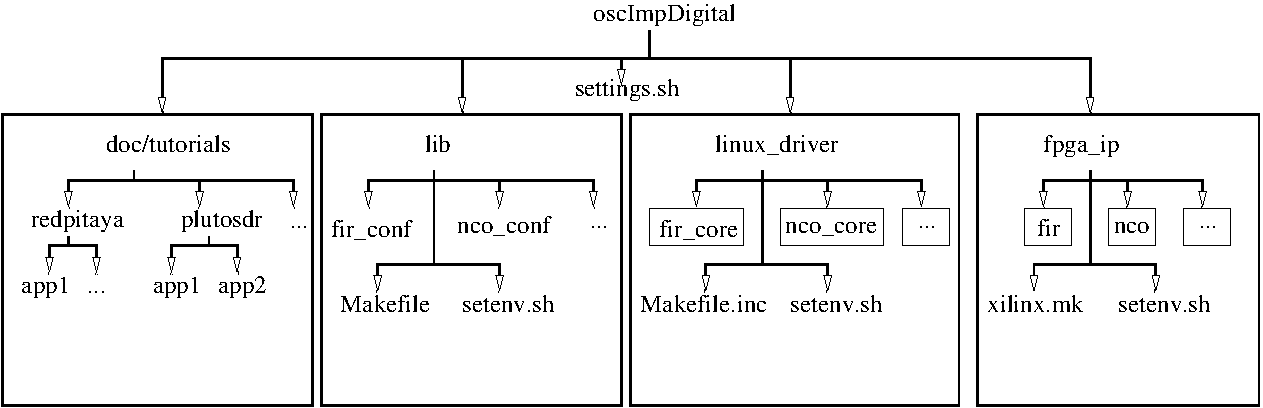
\includegraphics[width=1.0\textwidth]{./img/structRepo}
}
%\frame{\frametitle{Structure}
%}
\frame{\frametitle{FPGA}
\begin{minipage}[t]{\linewidth}
\begin{minipage}{0.6\linewidth}
Algorithms or utilities functions.

Developer aspect:
\begin{itemize}
\item normalize interfaces between blocks
\item isolation between implementation and communication
\end{itemize}

End user aspect:
\begin{itemize}
\item 0, 1 or more interface to connect;
\item AXI interface automatically connected.
\end{itemize}
\end{minipage}
\begin{minipage}{0.35\linewidth}
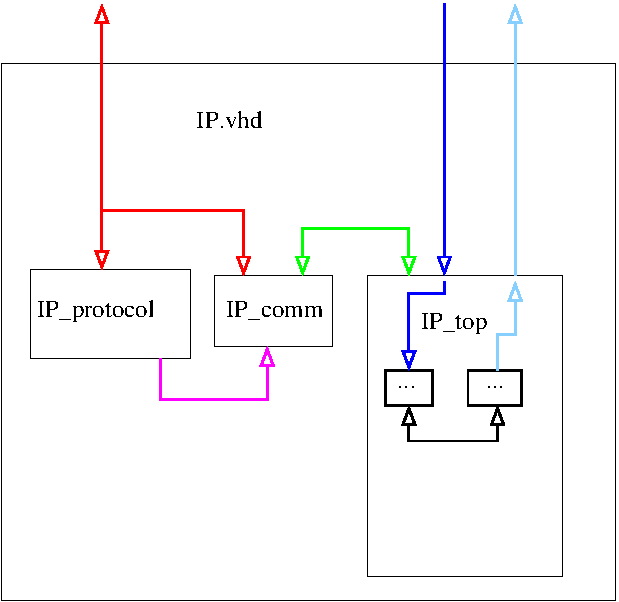
\includegraphics[width=1.2\textwidth]{./img/structureIp}
\end{minipage}
\end{minipage}
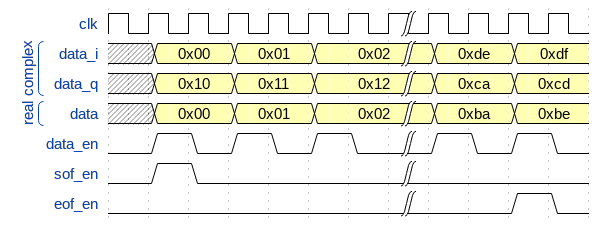
\includegraphics[width=0.9\textwidth]{./img/displayIf}
}
%\frame{\frametitle{CPU: environment}
%{\bf Char device drivers} to add abstraction, GNU/Linux hierarchy compliance and
%communication improvement:
%\begin{itemize}
%\item 1 IP with communication $\Rightarrow$ 1 (or more) driver(s);
%\item a {\tt core} driver knows how to communicate with an IP but not where;
%\item {\tt device tree overlay} used to provide which drivers must be probed and
%base address for each of them;
%\end{itemize}
%TODO $\Rightarrow$ IIO integration
%
%{\bf libraries} to simplify some common and long (number of line) tasks.
%}

\frame{\frametitle{Project structure}

\begin{itemize}
\item TCL script or GUI generated FPGA design
\item devicetree ({\tt .dts}) provides which driver must be used and base addresses;
\item {\tt Makefile} to cross-compile application and generate the {\tt dtbo} from dts
\item {\tt applicationName\_us.sh}: a shell script used to flash FPGA, load devicetree
and drivers;
\item {\tt main.c}: user application
\end{itemize}

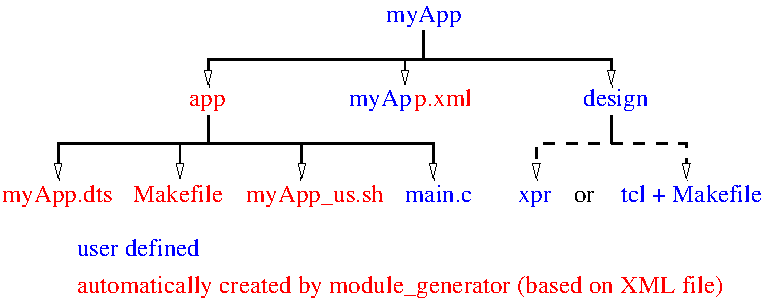
\includegraphics[width=1.0\textwidth]{img/structApp.pdf}
}

\begin{frame}[containsverbatim]
\frametitle{CPU: module\_generator}
\begin{itemize}
\item Used to generate some files in app directory.
\item use an XML file for design's informations.
\end{itemize}

{\small \verb!module_generator -dts myApp.xml!}

\hspace{-0.6cm}
%\begin{columns}[t]
%\begin{column}{0.57\textwidth}
%myApp.xml
%\vspace{-0.2cm}
{\footnotesize \begin{verbatim}
<?xml version="1.0" encoding="utf-8"?>
<project name="tutorial5" version="1.0">
  <options>
    <option target="makefile" name="USE_STATIC_LIB">1</option>
    <option target="makefile" name="LDFLAGS">-liio</option>
  </options>
  <ips>
    <ip name ="dataComplex_to_ram" >
      <instance name="data1600" id = "0"
        base_addr="0x43c00000" addr_size="0xffff" />
    </ip>
    <ip name ="nco_counter">
      <instance name="nco" id = "0"
        base_addr="0x43c10000" addr_size="0xffff" />
    </ip>
  </ips>
</project>
\end{verbatim}
}
\end{frame}

\begin{frame}[fragile]\frametitle{Application to GPS decoding}

\begin{itemize}
\item
TCL scripts define the processing functions, their settings and how they are 
connected to each other
\item Zynq on the PlutoSDR $\Rightarrow$ Xilinx Vivado (despite platform
independence of OscimpDigital)
\end{itemize}

\begin{center}
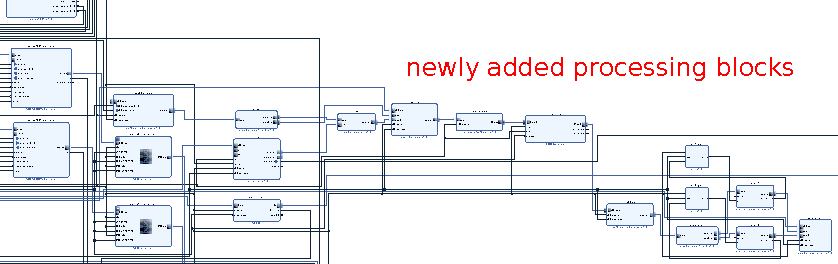
\includegraphics[width=1.04\linewidth]{2xcorr_2PRN_NCO_crop.pdf}
{\footnotesize Dual PRN generator and cross-correlation with the received datastream frequency
transposed using the NCO.\par}
\end{center}

\vfill
{\bf 22~s on Zynq PL} (limited by the FPGA area limiting the number of parallel correlations) v.s {\bf 108~s on 2.6 GHz PC} (GNU/Octave)
\end{frame}

\begin{frame}[fragile]\frametitle{Conclusion}

\begin{minipage}[t]{\linewidth}
\begin{minipage}{.65\linewidth}
{\footnotesize
\begin{itemize}
\item OscimpDigital as a {\bf flexible framework} 
for assembling signal processing
blocks on the FPGA in charge of collecting radiofrequency data
\item Platform {\bf independence} (useful investment for Intel/Altera SoC as well)
\item {\bf Consistent} IP--Linux kernel module--library--userspace application
\item Application to GPS decoding (dual channel, acquisition step) as SatCom
demonstration
\item {\bf Perspective}: port to ADRV9361 (Zynq 7035 $\gg$ 7010)
\end{itemize}
}
\vfill
\fbox{\parbox{\linewidth}{
Users {\bf not familiar with VHDL will benefit} from this framework since functional
processing blocks are provided
}}
\end{minipage}
\begin{minipage}{.34\linewidth}
~~~\includegraphics[width=\linewidth]{A4logos.png}

~~~~~~{\bf\footnotesize EU GNU Radio Days}
\end{minipage}
\end{minipage}

\vspace{0.1cm}
\noindent{\bf Resources:}

{\footnotesize
{\url{https://github.com/trabucayre/redpitaya}} (Buildroot BR2\_external)

{\url{https://github.com/oscimp/PlutoSDR}} (Buildroot BR2\_external)

{\url{https://github.com/oscimp/oscimpDigital}} (IP, driver, lib, tools \& doc)
}

\vfill
\noindent{Clone repository and submodules:}

{\footnotesize
{\verb!git clone --recursive https://github.com/oscimp/oscimpDigital.git!}
}
\end{frame}

\end{document}
